\chapter{Probabilistic programming}

\section{What is it ?} \label{PPL_def}
At a high level, \glspl{PPL} are \gls{PL} techniques to abstract inference algorithms from statistics such that they apply automatically and correctly to the broadest possible set of model-based reasoning applications.

A bit more precisely, Probabilistic programming systems \cite{Goodman:2012uq,dippl,Mansinghka:2014ty,wood-aistats-2014} represent generative models as programs written in a specialized language that provides syntax for the definition and conditioning of random variables.

Indeed, ``probabilistic programs are usual functional or imperative programs with two added constructs: 
(1) the ability to draw values at random from distributions, and 
(2) the ability to condition values of variables in a program via observations.'' \cite{Gordon:2014:PP:2593882.2593900}

Probabilistic programs define probability distributions over sequences of values, implicitly by means of program execution.

\section{Why is it useful ?}
For data science practitioners, statistical inference is typically just one step in a more elaborate analysis workflow. The first stage of this work involves data acquisition, preprocessing and cleaning. This is often followed by several iterations of exploratory model design and testing of inference algorithms. Once a sufficiently robust statistical model and a corresponding inference algorithm have been identified, analysis results must be post-processed, visualized, and in some cases integrated into a wider production system.

The main goal of \glspl{PPL} is to increase productivity. 
The code for models written with these systems is generally concise, modular, and easy to modify or extend.
Thus, one of the savings is to be found in the amount of code that needs to written in order to prototype and develop models.

Secondly, \glspl{PPL} remove the burden of having to develop inference code for each new model which is error-prone and time consuming.
This is done by providing a modeling language abstraction layer in which developers can denote their models.  Once denoted, generic inference is provided for free.

\section{Existing languages} \label{PPL_history}

The first generation of \glspl{PPL} had limitation in the range of models that could be represented and in which inference could be performed.
BUGS \cite{Bugs} and STAN \cite{Stan} can only work with graphical models.
Similarly, Factorie \cite{Factorie} and Infer.NET \cite{InferNET} only handle factor graphs.
These so-called \textit{First-Order} \gls{PPLs}, can only represent finite dimensional model and have bounded loops.

On the other hand, \textit{High Order \gls{PPLs}} which arrived a bit before the 2010s, are Turing complete, allow complex control flow, including stochastic recursion, thus can denote infinite dimensional objects.
%They are easy to program in, natural to express certain models, but it is hard to perform inference in these \glspl{PPL}. 
Anglican \cite{wood-aistats-2014}, Venture \cite{Mansinghka:2014ty}, Church \cite{Goodman:2012uq} and WebPPL \cite{dippl} are \textit{High Order \gls{PPLs}}.

\begin{figure}[h!]
\centering
    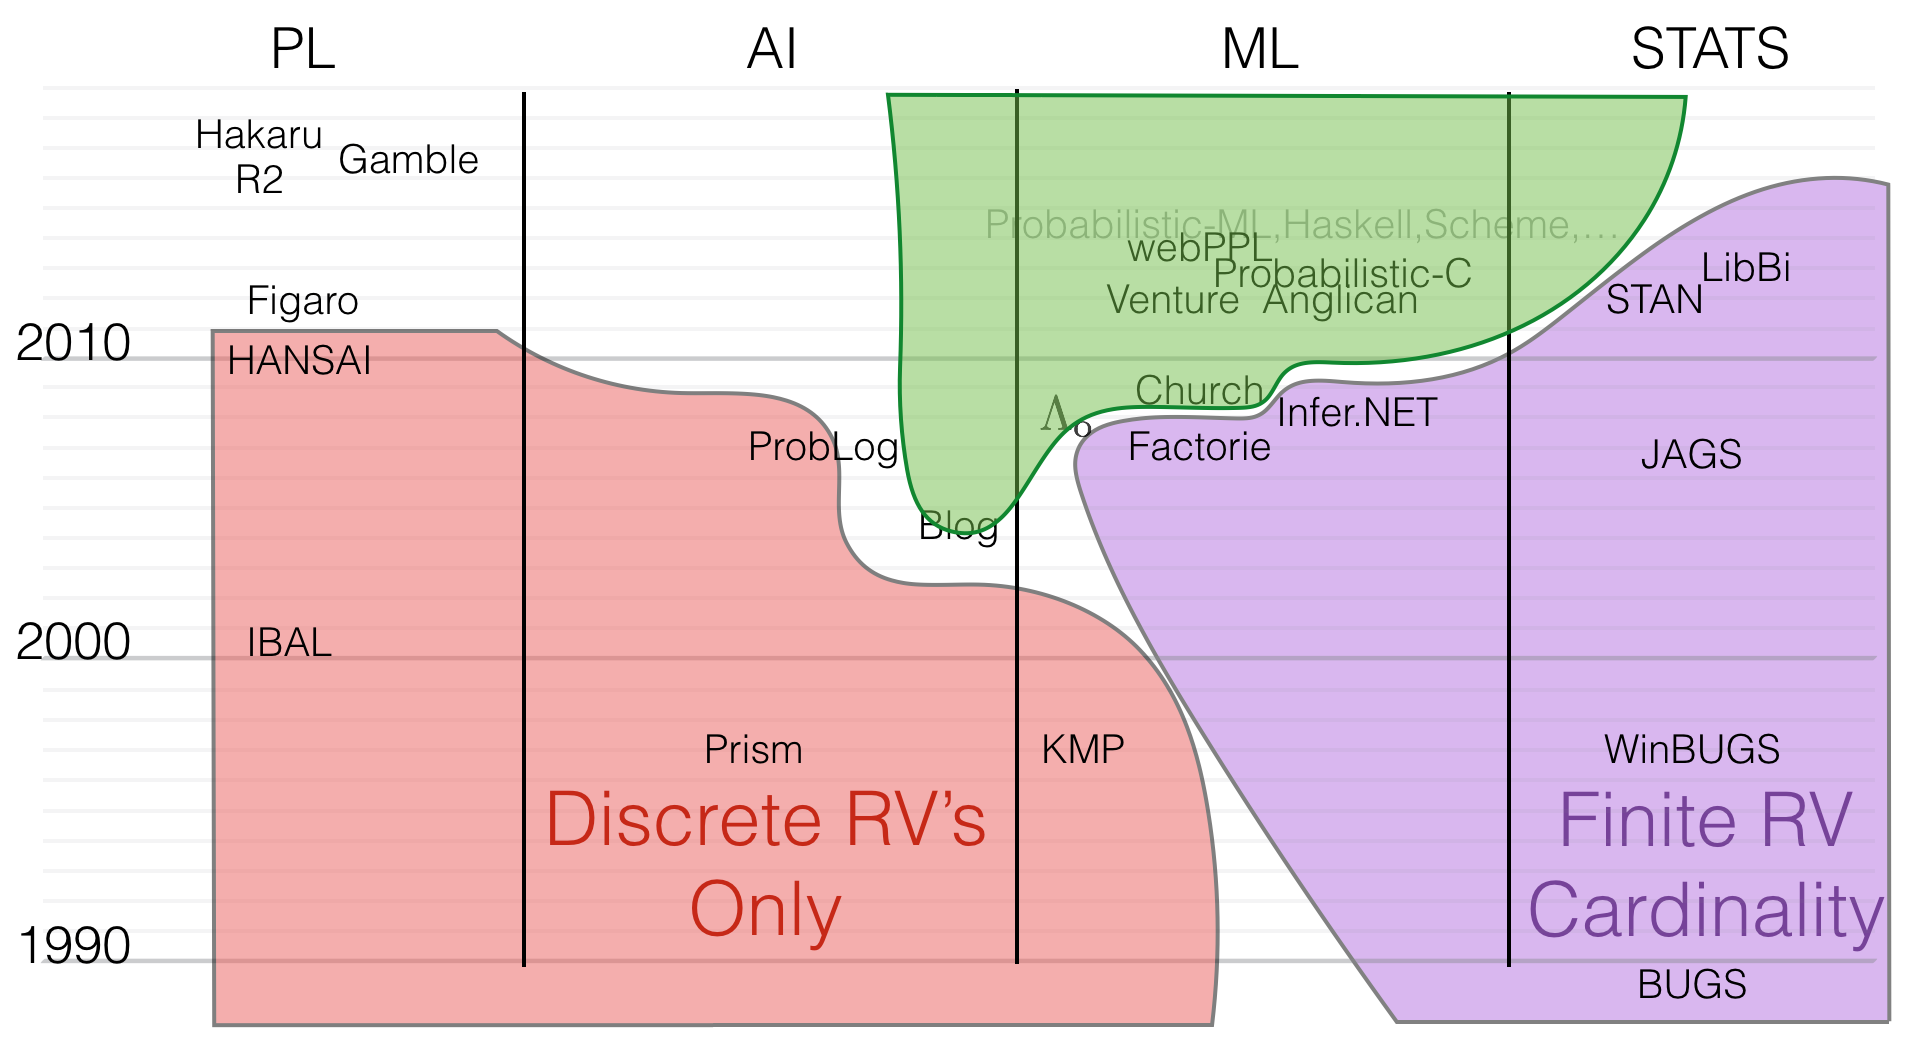
\includegraphics[width=0.9\linewidth]{ppls.png} 
    \caption{First-order and high-order \glspl{PPL}. Source: http://www.robots.ox.ac.uk/~fwood.}
    \label{fig:ppls} 
\end{figure}

Figure \ref{fig:ppls} shows a map of existing \glspl{PPL}, with first-order ones being in red and purple (bottom left/right), and high-order ones in green (top).
On one side, first-order \glspl{PPL} are quite restrictive since the spectrum of models that can be represented is limited to finite dimensional models, but inference can be performed efficiently.
On the other side, high-order \glspl{PPL} are more flexible but the task of writing efficient inference algorithm is harder.
There is therefore a trade-off between flexibility and efficiency, and the restrictions of first-order \glspl{PPL} are a design choice.

Recently, a new \gls{PPL} named Edward \cite{Edward} has been developed. It is different from the classical \glspl{PPL} since it focuses on \gls{VI} and Hamiltonian methods.


\section{Design}

Probabilistic programs denote probabilistic generative models as programs that include \texttt{sample} and \texttt{observe} statements (see Listing \ref{code:example_turing}). Both \texttt{sample} and \texttt{observe} are functions that specify random variables in this generative model using probability distribution objects as an argument, while \texttt{observe}, in addition, specifies the conditioning of this random variable upon a particular observed value in a second argument. These observed values induce a conditional probability distribution over the execution traces whose approximations and expected values we aim to characterize by \textit{performing inference}. \\

\begin{lstlisting}[caption={Example of a Turing.jl model},captionpos=b,label=code:example_turing]
@model model(y) = begin
  x = sample(Bernoulli(.75))
  mu = x ? 2 : 0
  observe(Gaussian(mu, 1), y)
  return x
end

sample(model(0.5), SMC(100))
\end{lstlisting}

A good way to understand this is to imagine the following interpreter of probabilistic programs. Starting from a fixed initial state, the interpreter runs the deterministic parts of a program according to the standard semantics, executes the \texttt{sample} statement by generating a random sample, and treats the \texttt{observe} statement by skip. More importantly, the interpreter keeps a log that records information about all the \texttt{sample} and \texttt{observe} forms encountered during execution. The information recorded for \texttt{sample} is a triple $(F, x, \alpha)$ of (i) a primitive probability distribution $F$, such as the standard normal, for which we have the probability density $f$ ; (ii) a value $x$ sampled from the distribution $F$ ; and (iii) an address $\alpha$ that uniquely and systematically identifies the random choice made. The information recorded for \texttt{observe} is a pair $(G,y)$ where $G$ is a primitive probability distribution with density $g$ and $y$ is an observed value.

An execution trace $\mbx$ is defined to be a sequence of triples $(F, x, \alpha)$ and $\mbx$ is said feasible if the trace is precisely the triple part of the log of some execution.
%Thus, an execution trace of a probabilistic program is obtained by successively executing the program deterministically, except when encountering \texttt{sample} statements at which point a value is generated according to the specified probability distribution $F$ and appended to the execution trace.
The observed values are denoted by $\mby := (y_j)_{j=1}^N$.

In most probabilistic programming systems any variable may be declared as being the output of a random procedure. Such variables can take different values in independent interpretations of the program. This leads to a ``many-worlds'' computational trace tree in which, at interpretation time, there is a branch at every random procedure application.

%Depending on the probabilistic program and the values generated at sample statements, the order in which the execution encounters sample statements as well as the number of encountered sample statements may be different from one trace to another.

A (almost-surely terminating) probabilistic program defines a probability distribution over finite feasible traces $\mbx$ with probability density $\pi(\mbx) := \gamma(\mbx) / Z$ where 

\begin{equation*}
\gamma(\mbx) := p(\mbx, \mby) = \prod_{i=1}^{|\mbx|}{f_{i}(x_i~|~x_{1:i-1})} \prod_{j=1}^{|\mby|}{g_j(y_j~|~x_{1:\tau(j)})}
\end{equation*}

where Z is the normalizing constant $Z := \int{\gamma(\mbx) d(\mbx)}$ and $\tau$ is a mapping from the index $j$ of the \texttt{observe} statement to the index of the last \texttt{sample} statement encountered before this \texttt{observe} statement during the execution of the program. Without any \texttt{observe} statement, the probability distribution over traces $\mbx$ is simply the prior

\begin{equation*}
p(\mbx) := \prod_{i=1}^{|\mbx|}{f_{i}(x_i~|~x_{1:i-1})}
\end{equation*}

\section{Inference}

Inference in probabilistic programming characterizes the conditional distribution of execution traces $\mbx$ given observed data $\mby$ assumed to have been generated by executing the probabilistic program.

Concretely, using the \texttt{sample} statements, the \gls{PPL}'s model first defines a so called prior distribution on these execution traces, and then it adjusts this prior distribution based on observations in data using the \texttt{observe} statement. Samples from this conditioned distribution (also called posterior distribution) can be obtained by running the model under one of the \gls{PPL}’s inference algorithms.


The inference algorithms may make random choices that do not correspond to any statements in the program, and decide which parts of the program code are executed and how often. Some inference algorithms re-run the program multiple times partially, from a certain point on, while reusing random choices made in the previous runs as much as possible.
Upon encountering a sample or observe record, the inference algorithm computes the updated program state and the value to be passed to the continuation. How the state is updated, the number of times the continuation is called, and the value passed to the continuation of sample depend on the inference algorithm executing the program.
Implementing an inference algorithm in \glspl{PPL} amounts to defining 
%an appropriate version of the infer function and 
checkpoint handlers for \texttt{sample} and \texttt{observe}.

Typically inference can be performed for any probabilistic program using one or more generic inference techniques provided by the system back end, such as Metropolis-Hastings \cite{Wingate:2011ul, Mansinghka:2014ty}, Hamiltonian Monte Carlo \cite{Stan}, expectation propagation \cite{InferNET}, and extensions of Sequential Monte Carlo \cite{vandeMeent:2015uk, Paige:2014tc, Wood:2015tr} methods.

\subsection{Use-case}
Even if as highlighted before, inference in \glspl{PPL} should be able to deal with arbitrary series of targets, for simplicity we will focus on a non-Markovian \gls{SSM}.

\Gls{SSM}s are probabilistic models over a set of latent variables $X_t \in \mathcal{X}_t, \forall t = 1 : T$ and observed variables $Y_t \in \mathcal{Y}_t , \forall t = 1 : T$ . We can further consider a model to be parameterized by $\theta \in \Theta$. The \gls{SSM} is then characterized by an initial density $\mu_\theta(x_1)$, a series of transition densities $f_{t,\theta}(x_t|x_{1:t-1})$, and a series of emission densities $g_{t,\theta}(y_t|x_{1:t})$.

\begin{equation*}
\begin{aligned}
& X_1 \sim \mu_\theta(\cdot) \\
& X_t|(X_{1:t-1} = x_{1:t-1}) \sim f_{t,\theta}(\cdot|x_{1:t-1}) \\
& Y_t|(X_{1:t} = x_{1:t}) \sim g_{t,\theta}(\cdot|x_{1:t}) \\
\end{aligned}
\end{equation*}

The joint density of the \gls{SSM} is then as follows

$$ \gamma_\theta(\mbx) := p_\theta(x_{1:T},y_{1:T}) = \mu_\theta(x_1) \prod_{t=2}^T f_{t,\theta}(x_t|x_{1:t-1}) \prod_{t=1}^T g_{t,\theta}(y_t|x_{1:t}) $$

We are free to choose any density for $\mu_\theta(x_1)$ and each $f_{t,\theta}(x_t|x_{1:t-1})$ and $g_{t,\theta}(y_t|x_{1:t})$. One is usually interested characterizing the posterior

$$ p_\theta(x_{1:T}|y_{1:T}) \propto p_\theta(x_{1:T},y_{1:T}) $$

Or expectations of some function $\phi$ under this posterior

$$ I(\phi) = \int \phi(x_{1:T}) p_\theta(x_{1:T}|y_{1:T}) dx_{1:T} $$

\subsection{Enumeration}
The easiest way one could think of to perform inference in a probabilistic program is via \textit{rejection sampling}. An execution trace can be thought of a \textit{path} in a \textit{tree} implicitly defined by a discrete model. This tree could then be explored using depth-first search, breadth-first search, or a probability-based priority queue. Then only the paths matching the observations $\mbx$ are retained and the others are rejected. These retained execution traces form the targeted posterior distribution.

\subsection{Markov Chain Monte Carlo}
Yet, for many models with large state spaces, enumeration is infeasible. This is particularly clear for models with continuous random variables, where the state space is infinite.
In the case of a large number of execution paths, one should avoid exploring all paths individually but only a subset of paths.

A popular way to estimate a difficult distribution is to sample from it by constructing a random walk that will visit each state in proportion to its probability. This class of algorithms are called \gls{MCMC}.
In our case, we are interested in random walk in the space of execution traces of a computation.

For discrete models, an easy way to a build random walk in the space of executions is to execute the probabilistic program by sampling variables at \texttt{sample} AND \texttt{observe} statements. The proposed execution trace $\mbx^\star$ shall then be rejected if at least one of the true observation $y_k$ does not match the associated generated observation $y \sim G$. If accepted, that means that this trace is one of the trace that can lead to the observations $\mby$, i.e. it belongs to the support of the targeted posterior distribution $p(\mbx|\mby)$. This method is called \textit{rejection sampling}. Yet, for highly dimensional space, this method will accept quite rarely a proposed trace. What is more, for continuous models, it will almost-surely never be accepted.

%However, this will not match the desired posterior distribution when the computation contains \texttt{observe} statements. The \gls{MH} algorithm gives a way to ‘patch up’ this random walk to get the right distribution.

A more complex Markov Chain needs to be built to have a reasonable acceptance rate.
Given a current trace $\mbx$ and score $p(\mbx)$, we proceed by reconsidering one random choice $x_k$.
Each \texttt{sample} statement is equipped with a proposal kernel $\mathcal{K}_k(x^\star|x, \psi)$, which is used to generate proposals to $x_k$. A random walk can the be built by (i) randomly choosing $k \in {1,\dots,|\mbx|}$, (ii) sample a new value $x_k^\star$ with $\mathcal{K}_k(x_k^\star|x_k, \psi)$ and (iii) re-run the program starting from $x_k$ which generate a new trace $\mbx^\star$. This new execution trace is accepted with probability

$$ 1 \wedge \frac{\gamma(\mbx^\star) \mathcal{K}_k(x_k|x_k^\star, \psi)}{\gamma(\mbx) \mathcal{K}_k(x_k^\star|x_k, \psi)} $$

This is better than our previous \gls{MH} algorithm, but when the chosen $k$ is close to $1$, it is almost as sampling from the prior since we only reuse the random choices made before the point of regeneration. So as to avoid having a small acceptance rate, it is generally better to make ‘smaller’ steps by reusing as many choices as possible. If we knew which sampled value was which, then we could look into the previous trace as the execution runs and reuse its values. That is, imagine that each call to sample was passed a (unique) name: \texttt{sample(name, dist)}. Then the \texttt{sample} function could try to look up and reuse values.
Notice that, in addition to reusing existing sampled choices, we add the name and mark whether this choice has been resampled. We must account for this in the \gls{MH} acceptance calculation.
We now hope to reuse most of the choices from the old trace in making a proposal.
This algorithm is called Lightweight \gls{MCMC} \cite{Wingate:2011ul}, and has been improved in \cite{Ritchie:2015tx}.

More generally, for an excellent introduction to \gls{MCMC} and particle inference in \glspl{PPL}, see \cite{dippl}.


\subsection{Importance Sampling} \label{IS}

\paragraph{Importance Sampling}
Importance sampling is an example of a Monte Carlo sampling scheme that provides approximately independent and identically distributed samples from a distribution of interest or target distribution, such as a posterior distribution, by generating a candidate sample from a proposal or importance distribution $q(\mbx|y_1,\dots,y_T)$.
The fact that the weights 
$w^k = \frac{p(\mbx, y_1,\dots,y_T)}{q(\mbx|y_1,\dots,y_T)} \propto \frac{p(\mbx|y_1,\dots,y_T)}{q(\mbx|y_1,\dots,y_T)}, \ \text{with} \ k \in 1,\dots,K$ can be computed is exploited, and samples from the target are obtained by sampling from the following weighted empirical distribution

$$ \hat{p}(\mbx|y_1,\dots,y_T) = \sum_{k=1}^K \bar{w}^k \delta_{\tilde{\mbx}^k} (\mbx)$$

where $\bar{w}^k = \frac{{w}^k}{\sum_{k=1}^K {w}^k}$ is the normalized weight and
$\delta_{z}$ is a Dirac measure centered on $z$.
The expectation $I(\phi)$ can also be approximated using

$$ \hat{I}(\phi) = \sum_{k=1}^K \bar{w}^k \phi(\tilde{\mbx})$$

% \begin{algorithm}  
%   \caption{ImportanceSampling(f, g)
%     \label{alg:is}}  
%   \begin{algorithmic}[1]  
%     \State  $\mu \gets 0_d$
%       \For{$t \gets 1 \textrm{ to } T$}  
%           \State  $\beta_t \gets 2 \log (\left| D \right| t^2 \pi^2 / 6 \delta)$
%     \State Choose $a_t \gets arg \max_i \mu_{t-1} + \sqrt{\beta_t} \sigma_{t-1}$
%     \State Observe $y_t = f(\mathbf{x}_t) + \epsilon_t$
%     \State $\mu_t = k_{t-1}(\mathbf{x})^T {(K_{t-1} + \sigma^2 I_d)}^{-1} y_t$
%     \State $k_t = k(\mathbf{x}, \mathbf{x}') - k_{t-1}(\mathbf{x})^T {(K_{t-1} + \sigma^2 I_d)}^{-1} k_{t-1}(\mathbf{x'}) $
%     \State $\sigma_{t}^2 = k_t(\mathbf{x},\mathbf{x})$
%       \EndFor  
%   \end{algorithmic}  
% \end{algorithm}

One problem with this method is that it is not easy to choose the proposal distribution $q$. A good proposal should share most of the support of the target distribution and have the same number of modes, i.e. it should be “close” to the target. A second problem is that it is a batch estimation method. To tackle this latter issue, in the next section, an extension to a sequential scenario is described.

\paragraph{Sequential Importance Sampling}
\gls{SIS} exploits the structure of a model by breaking down the overall inference problem into a series of target distributions which get incrementally closer to the distribution of interest.
These targets are then approximated by propagating a population of samples known as particles. If each intermediary target is kept similar to its predecessor, approximating one target given the last forms a significantly simpler problem than the overall inference.
Breaking the overall inference problem into a series of intermediate distributions makes the design of proposals easier since they must now be of the form $q(x_t|x_{1:t-1},y_{1:t})$ instead of $q(x_{1:T}|y_{1:T})$.

More formally, \gls{SIS} performs approximate inference on a sequence of target distributions
$\left(\pi_t(x_{1:t}) \right)_{t=1}^T$ of increasing spaces 
$\left(\mathcal{X}_1 \times \dots \times \mathcal{X}_t \right)_{t=1}^T$.
In the context of \glspl{SSM}, the target distributions are taken to be
$\left(p_\theta(x_{1:t}|y_{1:t}) \right)_{t=1}^T$.
At each time step $t$, we have a set of $K$ particles $\left(\tilde{x}_{1:t}^k \right)_{t=1}^T$,
corresponding to samples of the latents, and respective particle weights $\left({w}_{t}^k \right)_{t=1}^T$.
Similarly to \gls{IS}, using these weighted particles, one can approximate each posterior
$p_\theta(x_{1:t}|y_{1:t})$.
In particular, the posterior for the complete model $p_\theta(x_{1:T}|y_{1:T})$ and the expectation $I(\phi)$ can be approximated using the following estimators

$$ \hat{p}(x_{1:T}|y_{1:T}) = \sum_{k=1}^K \bar{w}_T^k \delta_{\tilde{x}_{1:T}^k} ({x}_{1:T})$$

$$ \hat{I}(\phi) = \sum_{k=1}^K \bar{w}_T^k \phi(\tilde{x}_{1:T})$$

where $\bar{w}_T^k = \frac{{w}_T^k}{\sum_{k=1}^K {w}_T^k}$ is the normalized weight.



Let's now focus on computing the particles' weights. The joint posterior can be written in the following factorised form

$$ p(x_{1:T}|y_{1:T}) = p(x_1) \prod_{t=2}^T p(x_t|x_{1:t-1},y_{1:t}) $$

The corresponding importance weights are thus

\begin{equation} \label{eq:IS_w}
\begin{aligned}
w_t =& \frac{p(x_{1:T}|y_{1:T})}{q(x_{1:T}|y_{1:T})} \\
w_t =& \frac{\mu(x_1) \prod_{t=2}^T p(x_t|x_{1:t-1},y_{1:t})}{q(x_1) \prod_{t=2}^T q(x_t|x_{1:t-1},y_{1:t})} \\
\end{aligned}
\end{equation}

The target distribution is the posterior distribution up to time $t$, which changes sequentially as we observe more data. This posterior distribution can be estimated recursively due to

\begin{equation} \label{eq:IS_p_rec}
p(x_{1:t+1}|y_{1:t+1}) = p(x_{1:t}|y_{1:t}) \times \frac{p(y_{t+1}|x_{1:t+1})p(x_{t+1}|x_{1:t})}{f(y_{t+1}|y_{1:t})} \\
\end{equation}

Substituting the numerator of Equation \ref{eq:IS_p_rec} in \ref{eq:IS_w} we obtain a recursive equation for the importance weight at time $t+1$

$$ w_{t+1} = w_{t} \times \frac{p(y_{t+1}|x_{1:t+1})p(x_{t+1}|x_{1:t})}{q(x_{t+1}|x_{1:t},y_{1:t+1})} $$


Even if we are not dealing with a \gls{SSM}, \gls{SIS} can be used as a general-purpose algorithm. The data are assumed to be observed sequentially so the observation’s index is the time index.


\paragraph{Sequential Monte Carlo} \label{SMC}

\begin{figure}[h!]
\centering
    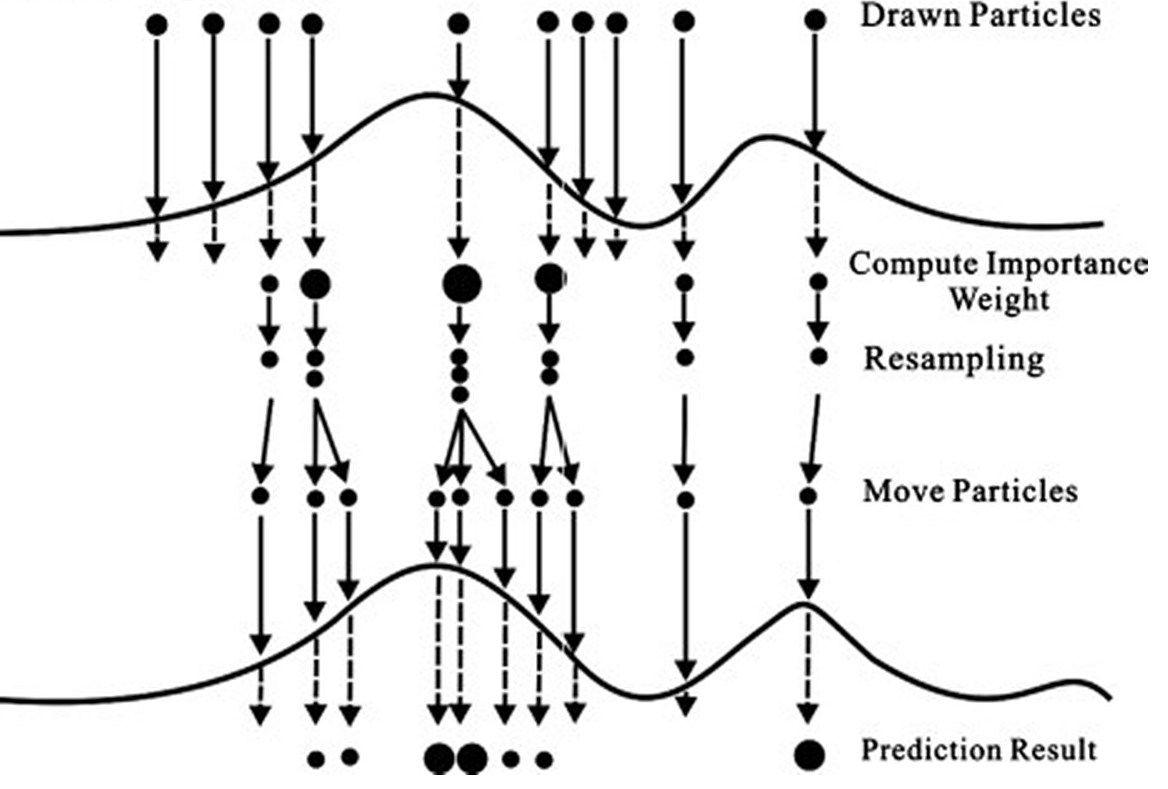
\includegraphics[width=0.7\linewidth]{particle_filter.png} 
    \caption{\acrlong{SMC}'s algorithm main steps. \\ Source: https://umbertopicchini.wordpress.com/2016/10/19/sequential-monte-carlo-bootstrap-filter.}
    \label{fig:smc} 
\end{figure}

The main problem with \gls{SIS} is that the weights become more skewed as the number of data points increases \cite{Anonymous:2001ue}, after a few steps only one particle will have a significant weight. To remedy this, a resampling step can be introduced which allows to eliminate particles with small weights and replicate particles with high weights, as illustrated in Figure \ref{fig:smc}.
The resampling step is achieved by, at each time step $t = 2, \dots , T$ ,
selecting the ancestor index $a^k_{t-1}$ for the $k$th particle from a discrete distribution 
$\mathcal{F} (\cdot|\bar{w}^1_{t-1},\dots, \bar{w}^K_{t-1})$
over parent indices ${1, \dots , K }$ with probabilities equal to the normalized weights at the previous time step $(\bar{w}^1_{t-1},\dots, \bar{w}^K_{t-1})$. The first resampling scheme introduced was the multinomial resampling for which $\mathbb{P}(a^k_{t-1} = i) \propto \bar{w}^i_{t-1}$. \cite{Douc:2005wa} provides a comparison of numerous different schemes for sampling from $\mathcal{F} (\cdot|\bar{w}^1_{t-1},\dots, \bar{w}^K_{t-1})$ that reduce the variance of the \gls{SMC} estimates compared with naïve multinomial resampling.
%We resample from the empirical posterior at step $t$
%$$ \hat{p}(x_{1:T}|y_{1:T}) = \sum_{k=1}^K \bar{w}_t^k \delta_{\tilde{x}_{1:T}^k} ({x}_{1:T})$$

This selection step can be introduced only occasionally or at every step of the algorithm.
If the selection step is to be performed occasionally, a possible criterion is when the \gls{ESS} is below a given threshold, which is a function of the number of particles, a popular choice is $0.5T$. The \gls{ESS} for the unnormalised weights is given by
$$ ESS_t = \frac{{\left( \sum_{k=1}^K{w_t^k} \right)}^2}{\sum_{k=1}^K{{w_t^k}^2}}$$

At step $t$, after the ancestors indices $\{a^k_{t-1}\}_{k=1}^K$ have been sampled, new $\{x_{t}^k\}_{k=1}^K$ are proposed according to $q(\cdot|x_{1:t-1},y_{1:t})$. Then, the particles' weights can be computed given
\begin{equation*} \label{eq:SMC_weights}
\begin{aligned}
w_{t}^k :=& \frac{p(x^k_{1:t},y_{t})}{p(x^k_{t}|x_{1:t-1}) q(x^k_{t}|x^k_{1:t-1},y_{1:t})}\\
=& \frac{p(y_{t}|x^k_{1:t})p(x^k_{t}|x^k_{1:t-1})}{q(x^k_{t}|x^k_{1:t-1},y_{1:t})}
\end{aligned}
\end{equation*}

\paragraph{\glspl{PPL} implementation of \gls{SMC}}

One a practical point of view, so as to handle particle algorithms, \glspl{PPL} must have the ability to stop the execution of the program at each time $t$ (more generally at each \texttt{observe} statement). Indeed, these \textit{chechpoints} are required by the \gls{SMC} algorithm for the resampling step.
Handling of checkpoints can be implemented through coroutines/co-operative multitasking (as in Turing \cite{Turing}), and parallel execution/preemptive multitasking, as well as through explicit maintenance of program continuations (as in \emph{Anglican} \cite{wood-aistats-2014} and \emph{WebPPL} \cite{dippl}).

Moreover, the proposals $q(\cdot|x_{1:t-1},y_{1:t})$ are generally implemented as being the prior $p(\cdot|x_{1:t-1})$ in \glspl{PPL}, i.e. the program is simply ran until an \texttt{observe} statement is encountered. Yet, by overriding the \texttt{sampler} statements, different proposals can be implemented. In the former case, the weights simplify to the likelihood; $w_{t}^k = p(y_{t}|x^k_{1:t})$, which can be computed at the \texttt{observe} statements. 

\subsection{Particle Markov Chain Monte Carlo} \label{PMCMC}
In a Bayesian setting, it is usual to consider the parameter $\theta$ in $p_\theta(x_{1:T}|y_{1:T})$ as a random variable by specifying a prior $p(\theta)$. In this subsection, we are therefore interested on algorithms targeting
$p(\theta, x_{1:T}|y_{1:T})$.
Let's think about \gls{MCMC} algorithms targeting the distribution $p(\theta, x_{1:T}|y_{1:T})$ which rely on sampling exactly from $p_\theta(x_{1:T}|y_{1:T})$, called ‘idealized’ algorithms.
Such algorithms are purely conceptual but a natural idea consists of approximating these idealized algorithms by using the output of an \gls{SMC} algorithm targeting $p_\theta(x_{1:T}|y_{1:T})$ using $K \ge 1$ particles as a proposal distribution for an \gls{MH} update.
Intuitively this could allow us to approximate with arbitrary precision such idealized algorithms while only requiring the design of low dimensional proposals for the \gls{SMC} algorithm.

A direct implementation of this idea is impossible as the marginal density of a particle that is generated by an \gls{SMC} algorithm is not available analytically but would be required for the calculation of the \gls{MH} acceptance ratio. Yet the \gls{SMC} algorithm yields an unbiased estimate of the marginal likelihood

$$ \hat{p}(y_{1:T}) = \prod_{t=1}^T \frac{1}{K} \sum_{k=1}^K w_t^k $$

which can be used for the calculation of the \gls{MH} acceptance ratio. 
These \gls{PMCMC} updates have been introduced in \cite{Andrieu:2010gc}.
The key feature of PMCMC algorithms is that they are in fact ‘exact approximations’ to idealized \gls{MCMC} algorithms targeting either $p(\theta, x_{1:T}|y_{1:T})$ in the sense that for any fixed number $N\ge1$ of particles their transition kernels leave the target density of interest invariant. 


\paragraph{Particle Marginal Metropolis-Hastings}
\gls{PMMH} makes use of the standard decomposition $p(\theta, x_{1:T}|y_{1:T}) = p(\theta | y_{1:T}) p_\theta(x_{1:T}|y_{1:T})$. 
It is natural to suggest the following form of proposal density for an \gls{MH} update:

$$ q\left( \theta^\star, x_{1:T}^\star | \theta, x_{1:T} \right) = q(\theta^\star|\theta) p_{\theta^\star}(x_{1:T}^\star|y_{1:T})$$

for which the proposed $x_{1:T}^\star$ is given by a \gls{SMC} algorithm targeting $p_{\theta^\star}(x_{1:T}|y_{1:T})$. Thus, the only degree of freedom of the algorithm (which will affect its performance) is $q(\theta^\star|\theta)$. The resulting \gls{MH} acceptance ratio is given by

$$ 1 \wedge \frac{p_{\theta^\star}(y_{1:T}) p(\theta^\star) q(\theta|\theta^\star)}{p_{\theta}(y_{1:T}) p(\theta) q(\theta^\star|\theta)} $$

\gls{PMMH} uses $\hat{p}(y_{1:T})$ to compute the acceptance ratio. It has been proven \cite{Andrieu:2010gc} that the \gls{PMMH} update leaves $p(\theta, x_{1:T}|y_{1:T})$ invariant and that under weak assumptions the \gls{PMMH} sampler is ergodic.


\paragraph{Particle Gibbs}
An alternative to the previous algorithm to sample from $p(\theta, x_{1:T}|y_{1:T})$ consists of using the Gibbs sampler which samples iteratively from $p(\theta|x_{1:T},y_{1:T})$ and $p_\theta(x_{1:T}|y_{1:T})$.
It is often possible to sample from $p(\theta|x_{1:T},y_{1:T})$ and thus the potentially tedious design of a proposal density for $\theta$ that is necessary in the \gls{PMMH} update can be bypassed.

It has been shown \cite{Andrieu:2010gc} that the naïve particle approximation to the Gibbs sampler where sampling from $p_\theta(x_{1:T}|y_{1:T})$ is replaced by sampling from an SMC approximation $\hat{p}_\theta(x_{1:T}|y_{1:T})$ does not admit $p(\theta, x_{1:T}|y_{1:T})$ as invariant density.

A valid particle approximation to the Gibbs sampler requires the use of a special type of \gls{PMCMC} update called the \textit{conditional} \gls{SMC} update. This update is similar to a standard \gls{SMC} algorithm but is such that a prespecified path $x^\star_{1:T}$ is ensured to survive all the resampling steps, whereas the remaining $N-1$ particles are generated as usual.

\paragraph{Particle Gibbs with Ancestor Sampling}
A drawback of \gls{PG} is that it can be particularly adversely affected by path degeneracy in the \gls{CSMC} step. Conditioning on an existing trajectory means that whenever resampling of the trajectories results in a common ancestor, this ancestor must correspond to this trajectory. Consequently, the mixing of the Markov chain for the early steps in the state sequence can become very slow when the particle set typically coalesces to a single ancestor during the \gls{CSMC} sweep.

\cite{Lindsten:2014uw} introduces \gls{PGAS}, which alleviates the problem with path degeneracy by modifying the original \gls{PG} kernel with a so-called \gls{AS} step.
The idea is to sample a new value for the index variable $a_t^N$ in an ancestor sampling step. While this is a small modification of the algorithm, the improvement in mixing can be quite considerable.
The task is to artificially assign a history to the partial path $(x^\star_{t:T})$ of the reference path.
This is done by connecting $(x^\star_{t:T})$ to one of the particles $(x^k_{1:t-1})$.
The ancestor index of the reference path $(x^\star_{t:T})$ at time $t$ $a^N_t \in \{1,\dots,K \}$ encodes the ancestry of this particle.

To assign a history to this partial path, first the following weights are computed

$$ \tilde{w}^k_{t-1|T} := {w}^k_{t-1} \frac{p((x^k_{1:t-1},x^\star_{t:T}), y_{1:T})}{p(x^k_{1:t-1}, y_{1:t-1    })}  $$

for $k = 1,\dots,K$. Then, $a^K_t$ is sampled via $\mathbb{P}\left( a^K_t = k \right) \propto \tilde{w}^k_{t-1|T}$.

\paragraph{Interacting Particle Markov Chain Monte Carlo}
\gls{IPMCMC} \cite{Rainforth:2016wq} is another way of tackling the path degeneracy issue.
In \gls{IPMCMC}, a pool of \gls{CSMC} and unconditional \gls{SMC} algorithms are ran as parallel processes (referred as nodes. After each run of this pool, successive Gibbs updates are applied to the indexes of the \gls{CSMC} nodes, such that the indices of the \gls{CSMC} nodes changes. Hence, the nodes from which retained particles are sampled can change from one \gls{MCMC} iteration to the next. This lets us trade off exploration (\gls{SMC}) and exploitation (\gls{CSMC}) to achieve improved mixing of the Markov chains.

\subsection{Hamiltonian samplers}

\paragraph{Hamiltonian Monte Carlo}
In \gls{HMC} \cite{HMC,Neal:2012uu}, a deterministic proposal process based on Hamiltonian dynamics is employed along with additional stochastic proposals that together provide an ergodic Markov chain capable of making large transitions that are accepted with high probability. The Hamiltonian makes use of the gradient of the joint distribution $p(\mbx, \mby)$ so as to construct better proposal.
% \textcolor{red}{speak about autodiff to compute this gradient ?}

\paragraph{No-U-Turn Sampler}
In \cite{NUTS}, the authors address the issue of choosing the two hyperparameters of \gls{HMC}: a step size $\epsilon$ and a desired number of steps $L$, since \gls{HMC}'s performance is highly sensitive on those.

First, \gls{NUTS} uses a recursive algorithm to build a set of likely candidate points that spans a wide swath of the target distribution, stopping automatically when it starts to double back and retrace its steps. The number of recursion calls is chosen to be the number of leapfrogs steps.
Moreover, if $\alpha_t$ is the Metropolis acceptance probability for iteration $t$ and $\delta$ is the desired average acceptance probability, we would like the statistic $H_t = \delta - \alpha_t$ to decreases towards $0$.
\gls{NUTS} achieves that goal by adaptively computing the step size using the dual averaging scheme of Nesterov \cite{Nesterov2009}, an algorithm for nonsmooth and stochastic convex optimization.

\paragraph{Stochastic Gradient Markov Chain Monte Carlo}
A recent focus has been on devising scalable variants of \gls{MCMC} algorithms that subsample the data and use stochastic gradients in place of full-data gradients in the dynamic simulations. Such algorithms are called \gls{SGMCMC} and a recipe has now been given \cite{SGMCMC} for deriving these schemes. \gls{SGMCMC} algorithms are well suited for online setting and can scale to big datasets.
\gls{SGLD} \cite{SGLD} and \gls{SGHMC} \cite{SGHMC} are examples of these schemes.
 
%Naive version is wrong (posterior is not the invariant distribution)
%friction term
 

\subsection{Variational Inference}

MCMC methods can be slow to converge and their convergence can be difficult to diagnose.
One class of alternative methods is provided by variational inference methods \cite{Jordan:1998ci,Ghahramani:2000:PAV:3008751.3008822}.
The basic idea of variational inference is to formulate the computation of a marginal
or conditional probability in terms of an optimization problem.
This (generally intractable) problem is then ``relaxed'', yielding a simplified optimization problem that
depends on a number of free parameters, known as variational parameters. Solving for the variational parameters gives an approximation to the marginal or conditional probabilities of interest.

To my knowledge, Edward \cite{Edward} is the only \gls{PPL} handling variational inference.

\section{Contributions}
During this internship I have taken the time to actually implement several inference algorithms, and by so, I contributed to two existing \glspl{PPL}.
Some only for the sake of learning more about sampling schemes and \glspl{PPL}, but others as specifically part of the project. 

First, I implemented \footnote{See \url{https://github.com/yebai/Turing.jl/tree/master/src/samplers}} both the \gls{SGLD} \footnote{See for instance, \gls{SGLD} applied to a Bayesian logistic regression at \url{https://github.com/yebai/Turing.jl/blob/master/example-models/sgld-paper/lr_sgld.jl}} and \gls{SGHMC} inference algorithms in Turing.jl \cite{Turing}, a \gls{PPL} based on Julia \cite{Bezanson:2017gd} and developed at the University of Cambridge.
Then, I implemented \footnote{See \url{https://github.com/blei-lab/edward/pull/728}} the Dual Averaging extension \cite{NUTS} of \gls{HMC} for Edward \cite{Edward}, a \gls{PPL} built on top of Tensorflow \cite{Tensorflow} by Blei's group \footnote{\url{http://www.cs.columbia.edu/~blei/}} at Columbia University.

More recently, I have worked on \gls{PMCMC} methods for Turing. \Gls{PMMH} \footnote{\url{https://github.com/yebai/Turing.jl/pull/339}} is implemented but not merged yet, and I am currently working on \gls{PGAS} and \gls{IPMCMC}. Consequently I became a \textit{Collaborator} of the Turing's repository.

I have also written a stick-breaking representation of the Dirichlet Process which inherits the Distribution.jl \footnote{\url{https://github.com/JuliaStats/Distributions.jl}} type so as to be easily used in Turing.
